\section{Prerequisiti}
Prima di speigare nftables si procede ad introdurre in maniera rigorosa iptables,
questo consentirà di comprendere meglio come mai nftables sia superiore.

\paragraph{netfiler}
\textit{netfilter} è il componente del kernel Linux che
``\textit{enables packet filtering, network address [and port] translation
(NA[P]T) and other packet mangling}'', il quale viene utilizzato mediante il
popolare programma iptables (ed \textit{ip6tables}, \textit{arptables},
\textit{ebtables}). Si tratta di una strumento molto
potente, che consente a qualsiasi dispositvo supportato dal kernel Linux
di diventare un firewall (o di compiere praticamente qualsiasi altra operazione
sui pacchetti in transito).\\
Sia netfilter sia iptables si scrivono senza maiuscole.


netfilter è composto da una serie di \textit{hook} a cui è possibile registrare
delle \textit{callback} che sono chiamate ogni volta che un pacchetto passa per
un certo hook.\\
Un pacchetto che entra in contatto con lo stack di rete di Linux transita per
diverse parti di esso in diversi momenti; un hook non è un altro che un \textit{punto} dello stack
in cui il pacchetto passa.
L'intero stack di rete offre numerosi hook, e non tutti sono disponibili in netfilter.
In particolare, gli hook disponibili per quest'ultimo sottosistema sono:
\begin{itemize}
  \item \texttt{NF\_IP\_PREROUTING}, raggiunto da tutti i pacchetti appena entrano nello
  stack di rete, la decisione di routing deve ancora essere presa.
  \item \texttt{NF\_IP\_LOCAL}, per i pacchetti dopo che sono stati \textit{routed}
  dal sistema e destinati al sistema locale.
  \item \texttt{NF\_IP\_FORWARD}: dopo che si è presa la decisione di routing,
  per pacchetti \textit{in transito} ad un altro sistema.
  \item \texttt{NF\_IP\_LOCAL\_OUT}: pacchetti creati localmente e destinati ad
  altri sistemi (quindi viene dopo la decisione di routing).
  \item \texttt{NF\_IP\_POSTROUTING}, raggiunto da tutto i pacchetti dopo che
  sono stati \textit{routed} e stanno per uscire dal sistema.
  \item \texttt{NF\_IP\_INGRESS} è un hook disponibile nelle versioni più recenti di
  Linux, avviene prima di \texttt{NF\_IP\_PREROUTING} per pacchetti in ingresso.
  E' utile per il cosìdetto ``\textit{early packet dropping}''.
\end{itemize}

\begin{figure}
  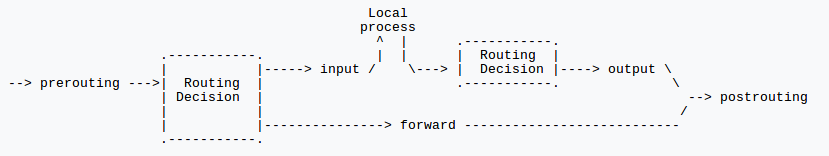
\includegraphics[scale=0.5]{img/NetfilterHooks}
  \caption[Hook di Netfiler]{Gli hook di Netfilter \textit{classici}. Tutti i
  pacchetti in arrivo passano per \texttt{PREROUTING}, viceversa quelli in
  uscita devono passare per forza per \texttt{POSTROUTING}.
  \url{https://wiki.nftables.org/wiki-nftables/index.php/Netfilter_hooks}}
  \label{fig:netfiler-hooks}
\end{figure}


\begin{figure}
  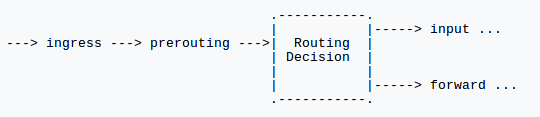
\includegraphics[scale=0.5]{img/NetfilterIngress}
  \caption[Hook \texttt{INGRESS}]{Hook \texttt{INGRESS} di Netfilter. E' l'hook
  che viene prima di tutti gli altri.
  \url{https://wiki.nftables.org/wiki-nftables/index.php/Netfilter_hooks}}
  \label{fig:ingress-hooks}
\end{figure}

\paragraph{iptables}
iptables è uno dei programmi userspace usati per registrare degli hook in netfilter e
specificare quale azioni devono essere eseguite.  Ciò che tipicamente si scrive
mediante iptables sono delle \textit{regole}, esse sono organizzate in
\textit{tabelle}, le quali a loro volta sono costituite da \textit{chain}. Esistono delle
tabelle predefinite:
\begin{itemize}
  \item \texttt{filter}: utilizzata per definire regole di firewalling
  \item \texttt{mangle}: utilizzata per \textit{packet alteration}
  \item \texttt{nat}: utilizzata la traduzione NAT/PAT
  \item \texttt{raw}: utilizzata principalmente operare sui pacchetti senza
  il connection tracking
  \item \texttt{security}: utilizzata in distribuzioni \texttt{SELinux}
\end{itemize}
E' possibile definire delle tabelle ulteriori.
Le chain predefinite sono:
\begin{itemize}
  \item \texttt{FORWARD} per pacchetti che passano attraverso
  il sistema
  \item \texttt{INPUT} per i pacchetti ricevuti e destinati al sistema locale
  \item \texttt{OUTPUT}: pacchetti generati dal sistema in uscita da esso
  \item \texttt{PREROUTING} per operare su pacchetti appena arrivano nello
  stack di rete
  \item \texttt{POSTROUTING} per lavorare su pacchetti quando stanno per uscire
  dal sistema.
\end{itemize}
Non tutte le tabelle hanno a disposizione tutte le chain, ad esempio nella tabella
di \texttt{nat} sono disponibili sono \texttt{PREROUTING} e \texttt{POSTROUTING}, mentre
in \texttt{filter} è possibile usare \texttt{INPUT}, \texttt{FORWARD}, \texttt{OUTPUT}.\\
Come si può dedurre dal nome delle chain, esse corrispondono agli hook di
netfilter:

\begin{table}[h]\label{tbl:iptables-chain}
  \begin{tabular}{|c|c|}
    \hline
    Hook & Chain \\
    \hline
    \hline
    \texttt{NF\_IP\_PREROUTING} & \texttt{PREROUTING}\\
    \hline
    \texttt{NF\_IP\_LOCAL} & \texttt{INPUT}\\
    \hline
    \texttt{NF\_IP\_FORWARD} & \texttt{FORWARD}\\
    \hline
    \texttt{NF\_IP\_LOCAL\_OUT} & \texttt{OUTPUT}\\
    \hline
    \texttt{NF\_IP\_POSTROUTING} & \texttt{POSTROUTING}\\
    \hline
  \end{tabular}
  \caption[La corrispondenza tra gli hook di netfilter e le chain di iptables.]
  {La corrispondenza tra gli hook di netfilter e le chain di iptables; si può notare
  come non sia possibile usare l'hook \texttt{NF\_IP\_INGRESS} perché non disponibile in
  iptables.}
\end{table}


\paragraph{Regole}
Le regole iptables sono composte da due parti: una parte detta di \textit{match}
nella quale si specificano i criteri per cui un pacchetto matcha o meno una regola,
ed una seconda di \textit{target} (indicato con l'opzione \texttt{-j}) che specifica quale
\textit{azione} compiere per quel pacchetto se vi è matching. Alcune tra i
target disponibili sono:
\begin{itemize}
  \item \texttt{ACCEPT} per accettare il pacchetto
  \item \texttt{DROP} per droppare il pacchetto, eliminandolo ed impedendo che
  prosegua nel suo attraversamento del kernel
  \item \texttt{REJECT} per droppare il pacchetto inviando un pacchetto
  \texttt{ICMP} al mittente
  \item \texttt{DNAT} per la traduzione NAT/PAT modificando l'indirizzo
  IP/porta destinazione
  \item \texttt{SNAT} per la traduzione NAT/PAT dell'indirizzo/porta sorgente.
\end{itemize}


Un'importante funzionalità offerta da netfilter è il tracking della connessione
in una tabelle di stato (nota come ``\textit{Connection Tracking}''), che è la base
per il NAT e statefull firewalling.\\
Infine, sono disponibili numerose estensioni sia per matching sia per target;
Ad esempio, esiste una versione di iptables
(\textit{iptables L7}) che aggiunge comprensione anche dei protocolli
applicativi\footnote{\url{http://l7-filter.clearos.com/start}}.
iptables viene usato con il protocollo IP versione 4 (e protocolli di livello
superiore che si appoggiano ad IPv4), se si vuole lavorare con protocolli
di livello 3 diversi, o protocolli di livello inferiore vi sono:
\begin{itemize}
  \item \texttt{arptables}: manipolazione del protocollo ARP
  \item \texttt{ebtables} per lavorare con protocolli di livello 2 (Ethernet)
  \item \texttt{ip6tables} per pacchetti che usano IPv6 come protocollo di rete.
\end{itemize}
